% *************
% INTRODUCCIÓN
% *************
\section*{INTRODUCCIÓN}
\addcontentsline{toc}{section}{INTRODUCCIÓN}

Los parqueaderos de vehículos en zonas urbanas son utilizados por la sociedad desde hace
muchos años, la creciente demanda de sistemas eficientes para la gestión de parqueaderos en
zonas urbanas ha impulsado el desarrollo de tecnologías avanzadas que optimicen el uso de los
espacios y mejoren la seguridad.

Actualmente, los métodos tradicionales, como las barreras automáticas o las cadenas de
seguridad, presentan limitaciones en términos de eficiencia, fiabilidad y personalización. Ante
esta problemática, surge la necesidad de implementar soluciones innovadoras que integren
tecnologías emergentes en los últimos años como la visión artificial y el aprendizaje profundo.

``El procesamiento de imágenes juega un papel vital en el reconocimiento de objetos y sus
características \cite{deshpande2020comparative}''.

``El seguimiento de vehículos con múltiples cámaras (MTMC) es esencial para el análisis
de tráfico y el mantenimiento de la seguridad \cite{tang2019cityflow}'', y junto con la
inteligencia artificial, permite una toma de decisiones más eficientes para favorecer
la gestión del establecimiento. Es decir, la automatización de la aplicación consigue
grandes beneficios, como en el ahorro de ciertos recursos económicos, cantidad y
calidad de los datos recolectados y permite una toma de decisiones efectiva.

Con este trabajo, se contribuye al desarrollo de tecnologías
inteligentes para la gestión de infraestructura urbana, brindando
soluciones eficientes, seguras y fáciles de implementar en el control de
acceso vehicular.

% *************
% ANTECEDENTES
% *************
\section*{ANTECEDENTES}
\addcontentsline{toc}{section}{ANTECEDENTES}

El crecimiento acelerado del parque automotor y la urbanización a nivel
mundial ha generado un aumento en la demanda de infraestructura idónea
para el estacionamiento de vehículos. Este fenómeno ha impulsado a
diversas ciudades y países a explorar soluciones tecnológicas
\cite{liu2023camera} que
permita gestionar de manera más eficiente los parqueaderos,
especialmente en zonas urbanas de mayor crecimiento. En este sentido,
los avances en visión artificial y aprendizaje profundo se han
posicionado como herramientas clave para automatizar y optimizar estos
procesos.

En Bolivia, la gestión de los parqueaderos ha sido un reto en
crecimiento, especialmente en la red troncal como La Paz, Cochabamba y
Santa Cruz, donde la expansión urbana ha generado una mayor demanda de
espacios de estacionamiento. Sin embargo, en comparación con otros
países de la región, Bolivia ha experimentado un desarrollo más limitado
en cuanto a la implementación de tecnologías avanzadas en este ámbito. A
nivel local, los sistemas de acceso y control vehicular siguen siendo
mayormente manuales o basados en tecnologías rudimentarios, como la
intervención humana.

En los últimos años, algunas empresas en el país han empezado a adoptar
tecnologías de reconocimiento de placas y cámaras de seguridad. Sin
embargo, se observa una limitada adopción documentada en el uso de aprendizaje
profundo para este propósito, lo que subraya la oportunidad de desarrollo e
innovación en este campo de la inteligencia artificial.

A nivel global, los sistemas inteligentes de control vehicular basados
en visión artificial y aprendizaje profundo han alcanzado un notable
grado de sofisticación, particularmente en países de Europa, Asia, y
Norteamérica. China y los Estados Unidos lideran la implementación de
estas tecnologías, para gestionar grandes volúmenes de tráfico y mejorar
la seguridad.
\subsection*{TRABAJOS DESARROLLADOS}
\addcontentsline{toc}{subsection}{TRABAJOS DESARROLLADOS}

\textbf{ANÁLISIS, DISEÑO E IMPLEMENTACIÓN DE UN SISTEMA DE CONTROL DE
INGRESO DE VEHÍCULOS BASADO EN VISIÓN ARTIFICIAL Y RECONOCIMIENTO DE
PLACAS EN EL PARQUEADERO DE LA UNIVERSIDAD POLITÉCNICA SALESIANA - SEDE
CUENCA}

Desarrollado por Alvares Duran Mayra Alejandra\cite{alvares2014control}, el presente
trabajo consiste en un sistema de reconocimiento de placas vehiculares
que utiliza algoritmos de Reconocimiento Óptico de Caracteres ROC o OCR,
mediante las librerías OpenCV, está desarrollado en lenguaje JAVA y se
encuentra basado en Inteligencia Artificial, esta herramienta recibe y
procesa las imágenes desde una cámara de video que se encuentra al
ingresar al parqueadero de la Universidad Politécnica Salesiana, sede
Cuenca.

\textbf{DISEÑO E IMPLEMENTACIÓN DE UNA METODOLOGÍA BASADA EN
INTELIGENCIA ARTIFICIAL CAPAZ DE CONTAR Y CLASIFICAR VEHÍCULOS EN LOS
ACCESO DE AEROPUERTOS Y DE RECONOCER VEHÍCULOS AEROPORTUARIOS}

Realizado por Martines Samper Aniceto José \cite{martines2022vehiculos} en la Universidad
Politécnica de Valencia (UPV), este proyecto se basa en realizar un
conteo y una clasificación automática de vehículos, capaz de
acoplarse a cualquier video de circulación. Particularizando un poco
más, este proyecto se va a centrar principalmente en la composición de
un algoritmo para el conteo y clasificación de vehículos en las entradas
de aeropuertos. Para efectuar este estudio, se ha trabajado con el
lenguaje de programación OpenCV. En este proceso, el programa irá evolucionando el programa
hasta poder conseguir un resultado óptimo, partiendo de una programación
más simple, pasando por métodos básicos de procesamiento de imagen y
finalizando en la implementación de redes neuronales (YOLO) para la
detección y clasificación de objetos.

\textbf{SISTEMA INTELIGENTE DE GESTIÓN DE TRÁFICO}

González Caballero Javier \cite{gonzalez2019sistema}, de la universidad
de Valladolid En este proyecto se propone un sistema alternativo capaz
de modificar en tiempo real la duración en verde o en rojo de los
semáforos según el flujo de vehículos y la presencia o no de peatones.
Para ello, se analiza la tecnología de control de los semáforos que
se emplea actualmente y las investigaciones realizadas.

\subsection*{INFORMACIÓN DOCUMENTAL Y ESTADÍSTICA}
\addcontentsline{toc}{subsection}{INFORMACIÓN DOCUMENTAL Y ESTADÍSTICA}

La información documental y estadística que sostiene el problema proviene de dos
fuentes verificables. La primera es el registro oficial del parque automotor que
publica el Instituto Nacional de Estadística (INE) a partir de los datos del
Registro Único para la Administración Tributaria Municipal (RUAT)
\cite{ine2026parqueautomotor}. La segunda es la campaña de grabación realizada en
el recinto de estudio, cuyos metadatos describen la cobertura temporal del material
analizado en este trabajo.

\textbf{Parque automotor.} El parque automotor registrado en Bolivia creció de
2,470,622 vehículos en 2023 a 2,583,319 en 2024 y 2,672,176 en 2025, con
variaciones anuales de $4{.}6$\,\% y $3{.}4$\,\% respectivamente. El departamento
de Oruro siguió la misma tendencia: 120,400 vehículos en 2023, 124,008 en 2024
y 127,285 en 2025 (Tabla~\ref{tab:parque_automotor}). El crecimiento sostenido
del parque vehicular aumenta la presión sobre los puntos de acceso de los
parqueaderos: un registro manual de placas atiende un vehículo por vez, de modo que
cada unidad adicional se traduce en espera en la barrera y en cola sobre la vía
pública.

\begin{table}[H]
    \centering
    \caption{Parque automotor registrado en Bolivia y en el departamento de Oruro.
    Fuente: INE, con base en el RUAT \cite{ine2026parqueautomotor}.}
    \label{tab:parque_automotor}
    \begin{tabular}{lrrr}
        \toprule
        \textbf{Año} & \textbf{Bolivia} & \textbf{Oruro} &
        \textbf{Variación anual en Oruro} \\
        \midrule
        2023 & 2,470,622 & 120,400 & --- \\
        2024 & 2,583,319 & 124,008 & $+3{.}0$\,\% \\
        2025 & 2,672,176 & 127,285 & $+2{.}6$\,\% \\*
        \multicolumn{3}{r}{\footnotesize\textit{Fuente: INE, con base en el RUAT}} \\*
        \bottomrule
    \end{tabular}
\end{table}

\textbf{Proyección.} Con tres observaciones anuales no se puede estimar un modelo
con intervalo de predicción defendible, pero sí una proyección mecánica que acote
el orden de magnitud. Aplicando la tasa de crecimiento anual compuesta del
departamento entre 2023 y 2025 ($2{.}82$\,\%) se obtienen 146,270 vehículos en
2030; aplicando la tasa nacional del mismo período ($4{.}0$\,\%) se obtienen
154,855. Una extrapolación lineal sobre los mismos datos arroja 144,498, dentro
del mismo orden. La Tabla~\ref{tab:proyeccion_parque} resume los dos escenarios.

\begin{table}[H]
    \centering
    \caption{Proyección del parque automotor de Oruro bajo dos escenarios de
    crecimiento. Elaboración propia a partir de la serie del INE
    \cite{ine2026parqueautomotor}. Es una extrapolación mecánica, no un
    pronóstico.}
    \label{tab:proyeccion_parque}
    \begin{tabular}{lrr}
        \toprule
        \textbf{Año} & \textbf{Escenario base ($2{.}82$\,\%)} &
        \textbf{Escenario alto ($4{.}0$\,\%)} \\
        \midrule
        2026 & 130,874 & 132,375 \\
        2027 & 134,564 & 137,669 \\
        2028 & 138,358 & 143,174 \\
        2029 & 142,259 & 148,900 \\
        2030 & 146,270 & 154,855 \\*
        \multicolumn{3}{r}{\footnotesize\textit{Fuente: Elaboración propia}} \\*
        \bottomrule
    \end{tabular}
\end{table}

Se trata de una proyección, no de un pronóstico: supone que la tasa reciente se
mantiene y no modela saturación del parque, cambios normativos ni crisis
económicas. Se incluye porque el orden de magnitud ---entre $144{,}000$ y $155{,}000$
vehículos en 2030--- es lo que importa para dimensionar un punto de acceso, no
porque permita predecir el valor exacto. La cifra observada sigue siendo la que
sostiene el problema; la proyección solo muestra hacia dónde crece.

\textbf{Campaña de grabación.} El material del estudio se recolectó en el recinto
entre el 16 de marzo y el 16 de mayo de 2026, con las cámaras de los accesos del
recinto.
La campaña comprende $276$ sesiones de una hora, una por hora grabada, distribuidas
en $39$ días. La Figura~\ref{fig:cobertura_grabacion} muestra las horas registradas
por día de la semana: la cobertura es pareja de lunes a sábado (entre $37$ y $52$
horas) y baja el domingo ($8$ horas). Esa distribución condiciona el alcance de los
resultados: las conclusiones sobre el domingo se limitan a la evidencia disponible
para ese día, mientras que el resto de la semana cuenta con material suficiente
para las mediciones que se reportan en el Capítulo~III. Ese capítulo detalla qué
subconjunto de este material se destinó a cada medición y qué horas quedaron fuera
de cada conjunto de prueba.

\begin{figure}[htbp]
    \centering
    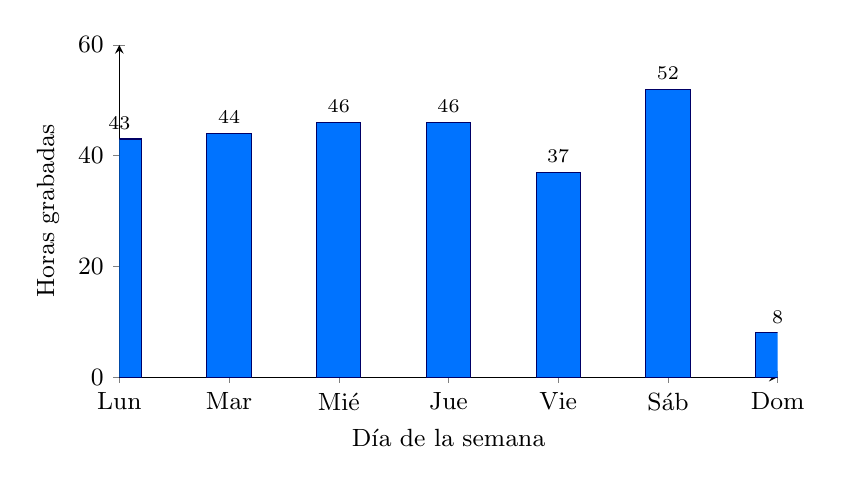
\begin{tikzpicture}
        \begin{axis}[
            ybar,
            width=0.82\textwidth,
            height=5.8cm,
            ymin=0, ymax=60,
            ylabel={Horas grabadas},
            xlabel={Día de la semana},
            symbolic x coords={Lun, Mar, Mié, Jue, Vie, Sáb, Dom},
            xtick=data,
            nodes near coords,
            every node near coord/.append style={font=\scriptsize},
            bar width=16pt,
            enlarge x limits=0.10,
            axis lines=left,
            tick label style={font=\small},
            label style={font=\small},
        ]
            \addplot[fill=blue!55!cyan, draw=blue!40!black] coordinates {
                (Lun, 43) (Mar, 44) (Mié, 46) (Jue, 46) (Vie, 37) (Sáb, 52) (Dom, 8)
            };
        \end{axis}
    \end{tikzpicture}
    \caption{Horas de grabación por día de la semana en el recinto de estudio,
    entre el 16 de marzo y el 16 de mayo de 2026. Fuente: metadatos de las
    sesiones registradas por las cámaras del recinto.}
    \label{fig:cobertura_grabacion}
\end{figure}

% ***********************
% SITUACIÓN PROBLEMÁTICA
% ***********************
\section*{SITUACIÓN PROBLEMÁTICA}
\addcontentsline{toc}{section}{SITUACIÓN PROBLEMÁTICA}

En los parqueaderos urbanos, el control de ingreso y salida de vehículos
se realiza mediante procedimientos manuales o semiautomáticos que requieren
la intervención de operadores para registrar y verificar la información
correspondiente. Esta práctica genera tiempos de atención variables, errores
en el registro y dificultades para disponer de información confiable sobre
los vehículos que ingresan y salen del recinto.

En el parqueadero, la ausencia de un mecanismo automatizado
para identificar las características de los vehículos limita el registro
sistemático de información como el tipo de vehículo, el color predominante
y la placa de matrícula. Asimismo, la falta de un registro asociado a la
fecha, hora, punto de acceso y sentido del evento dificulta la trazabilidad
de los movimientos vehiculares y la generación posterior de información
estadística.

A lo anterior se suma una limitación en el control de acceso: la
identificación de los vehículos y la verificación de su autorización no se
realizan de manera automatizada, lo que dificulta la detección oportuna de
vehículos no autorizados y la disponibilidad de evidencia digital auditable.

A esto se suma que las condiciones de captura de las cámaras --variaciones
de iluminación, distancia, ángulo de observación, oclusiones parciales y
visibilidad de las placas-- pueden afectar la identificación automática de los
vehículos. Estas condiciones reales del entorno deben ser consideradas
durante la construcción y evaluación de los modelos de visión artificial.

Ante esta situación, se plantea el desarrollo de un sistema basado en visión
artificial y aprendizaje profundo que automatice la identificación de los
vehículos en los puntos de acceso, reconozca su tipo, color predominante y
placa de matrícula, registre los eventos de ingreso y salida, y almacene la
información generada para su consulta y análisis.

% ***************************
% PLANTEAMIENTO DEL PROBLEMA
% ***************************
\section*{PLANTEAMIENTO DEL PROBLEMA}
\addcontentsline{toc}{section}{PLANTEAMIENTO DEL PROBLEMA}

En el control de acceso vehicular de los parqueaderos, los procedimientos
manuales o semiautomáticos pueden generar errores de registro, dificultades para
ejecutar el seguimiento de los vehículos y limitaciones para disponer de
información confiable sobre los eventos de ingreso y salida. La ausencia de
mecanismos automatizados para identificar las características de los vehículos
también dificulta la revisión de los accesos y la generación de información
histórica para el análisis de la operación del recinto.

En el parqueadero, esta problemática se relaciona con la necesidad de
identificar automáticamente los vehículos considerando su tipo, color
predominante y placa de matrícula, registrar la fecha, hora, cámara y sentido
correspondiente al evento, y disponer de esta información para consulta,
seguimiento y análisis estadístico.

En este contexto, el desarrollo de técnicas de visión artificial y aprendizaje
profundo ofrece la posibilidad de automatizar parte del proceso de identificación
vehicular mediante el procesamiento de imágenes y video. Sin embargo, el
desempeño del sistema depende de factores como las condiciones de iluminación,
el ángulo y distancia de captura, las características de las placas y la calidad
de las imágenes obtenidas en el entorno de estudio.

Por tanto, el problema de investigación se centra en determinar en qué medida un
sistema basado en visión artificial y aprendizaje profundo puede automatizar la
identificación de vehículos y el registro de sus eventos de ingreso y salida,
manteniendo un desempeño adecuado bajo las condiciones de captura del parqueadero.

En este contexto, se formula la siguiente pregunta de investigación:
\begin{quote}
    ¿En qué medida un sistema basado en visión artificial y aprendizaje profundo
    puede automatizar la identificación de los vehículos, mediante el
    reconocimiento de su tipo, color predominante y placa de matrícula, así como
    el registro de sus eventos de ingreso y salida, bajo las condiciones de
    captura del parqueadero?
\end{quote}

\section*{OBJETO DE ESTUDIO}
\addcontentsline{toc}{section}{OBJETO DE ESTUDIO}

El proceso de control de acceso e identificación vehicular en parqueaderos urbanos.

\section*{OBJETIVOS}
\addcontentsline{toc}{section}{OBJETIVOS}

\subsection*{OBJETIVO GENERAL}
\addcontentsline{toc}{subsection}{OBJETIVO GENERAL}

Desarrollar un sistema inteligente para la gestión automatizada del control de
acceso vehicular en un parqueadero, mediante técnicas de visión artificial y
aprendizaje profundo, que permita identificar el tipo, color predominante y placas
de los vehículos, registrar los eventos de ingreso y salida y generar información 
para el seguimiento y análisis de la operación del recinto.

\subsection*{OBJETIVOS ESPECÍFICOS}
\addcontentsline{toc}{subsection}{OBJETIVOS ESPECÍFICOS}

\begin{itemize}
    \item
        Analizar las condiciones de operaciones del parqueadero, las características
        de los puntos de acceso y los requerimientos técnicos y funcionales del
        sistema, considerando las condiciones de captura de las cámaras,
        para establecer los criterios de diseño de la solución propuesta.
    \item
        Construir y preparar un conjunto de datos representativos de las condiciones
        reales del parqueadero, mediante la selección, extracción, organización y
        anotación de imágenes de vehículos, considerando sus categorías, color
        predominante y placas, para el entrenamiento y evaluación de los modelos
        de visión artificial.
    \item
        Adaptar y entrenar modelos de aprendizaje profundo para la detección
        e identificación del tipo y color predominante de los vehículos, así como
        para la localización de sus placas, utilizando el conjunto de datos
        construido y evaluando su desempeño mediante métricas apropiadas.
    \item
        Desarrollar y entrenar un modelo de reconocimiento óptico de caracteres orientado
        a la lectura de placas vehiculares, empleando datos correspondientes
        al formato de las matrículas presentes en el contexto del estudio, y
        evaluar su desempeño bajo diferentes condiciones de visibilidad.
    \item
        Integrar los modelos de visión artificial en un sistema de gestión
        que permita registrar los vehículos identificados y sus eventos de ingreso
        y salida, asociando la información obtenida con la fecha, hora y cámara
        correspondiente, y proporcionando mecanismos para su consulta y visualización.
    \item
        Evaluar el desempeño del sistema desarrollado mediante pruebas experimentales
        en condiciones representativas del entorno de estudio, considerando la
        precisión de la detección e identificación de vehículos y placas, la correcta
        determinación de los eventos de ingreso y salida y el rendimiento computacional
        del modelo antes y después de aplicar técnicas de optimización.
\end{itemize}

% ****************
% CAMPO DE ACCIÓN
% ****************
\section*{CAMPO DE ACCIÓN}
\addcontentsline{toc}{section}{CAMPO DE ACCIÓN}

La automatización del proceso de identificación y registro de vehículos en los
puntos de acceso de un parqueadero, mediante técnicas de visión computacional y
aprendizaje profundo, considerando el reconocimiento de su tipo, color
predominante y placa de matrícula, así como el registro de los eventos de
ingreso y salida.

% **********
% HIPÓTESIS
% **********
\section*{HIPÓTESIS}
\addcontentsline{toc}{section}{HIPÓTESIS}

\textbf{Hipótesis general ($H_1$):}

El sistema de gestión inteligente de parqueaderos basado en visión artificial y
aprendizaje profundo alcanza los criterios de desempeño establecidos para la
detección e identificación de vehículos, el reconocimiento de placas de
matrícula y la determinación de los eventos de ingreso y salida, bajo las
condiciones de captura del entorno de estudio.

\textbf{Hipótesis nula ($H_0$):}

El sistema de gestión inteligente de parqueaderos basado en visión artificial y
aprendizaje profundo no alcanza los criterios de desempeño establecidos para la
detección e identificación de vehículos, el reconocimiento de placas de
matrícula y la determinación de los eventos de ingreso y salida, bajo las
condiciones de captura del entorno de estudio.

$H_{1{.}1}$: El modelo de detección de vehículos alcanza un mAP@50 igual o superior
al 80 \% bajo las condiciones de captura del entorno de estudio.

$H_{0{.}1}$: El modelo de detección de vehículos no alcanza un mAP@50 del 80 \%
bajo las condiciones de captura del entorno de estudio.

$H_{1{.}2}$: El modelo de identificación del tipo de vehículo alcanza un F1-score
macro igual o superior al 85 \% bajo las condiciones de captura del entorno de
estudio.

$H_{0{.}2}$: El modelo de identificación del tipo de vehículo no alcanza un
F1-score macro del 85 \% bajo las condiciones de captura del entorno de estudio.

$H_{1{.}3}$: El modelo de identificación del color predominante alcanza un F1-score
macro igual o superior al 85 \% bajo las condiciones de captura del entorno de
estudio.

$H_{0{.}3}$: El modelo de identificación del color predominante no alcanza un
F1-score macro del 85 \% bajo las condiciones de captura del entorno de estudio.

$H_{1{.}4}$: El sistema de reconocimiento de placas alcanza simultáneamente un
Recall igual o superior al 90 \% en la detección de las placas y una exactitud
por carácter igual o superior al 90 \% en el reconocimiento de las matrículas,
bajo las condiciones de visibilidad del entorno de estudio.

$H_{0{.}4}$: El sistema de reconocimiento de placas no alcanza simultáneamente los
valores mínimos establecidos para la detección y el reconocimiento de las
matrículas bajo las condiciones de visibilidad del entorno de estudio.

$H_{1{.}5}$: El sistema determina correctamente los eventos de ingreso y salida de
los vehículos con una exactitud igual o superior al 90 \% bajo las condiciones
de operación del parqueadero.

$H_{0{.}5}$: El sistema no alcanza una exactitud del 90 \% en la determinación de
los eventos de ingreso y salida bajo las condiciones de operación del parqueadero.

\subsection*{CRITERIO DE EVALUACIÓN DE LA HIPÓTESIS}
\addcontentsline{toc}{subsection}{CRITERIO DE EVALUACIÓN DE LA HIPÓTESIS}


La contrastación de la hipótesis se realizó mediante pruebas experimentales
sobre un conjunto de datos de prueba independiente de los datos utilizados para
el entrenamiento de los modelos. El conjunto de prueba contiene muestras
representativas de las condiciones de captura del parqueadero, incluyendo
variaciones de iluminación, visibilidad, distancia, ángulo de captura y
oclusiones presentes en el entorno de estudio.

La evaluación se realizó de forma independiente para cada componente del
sistema. En todo el documento se emplean \emph{precisión} (\textit{precision}),
\emph{exhaustividad} (\textit{recall}) y \emph{exactitud} (\textit{accuracy});
cuando una métrica se cita con su nombre en inglés, corresponde al mismo
indicador. Los criterios aplicados son los siguientes:

\begin{itemize}
    \item \textbf{Detección de vehículos:} se utilizó como indicador principal
        el mAP@50, considerando como criterio mínimo de cumplimiento un valor
        igual o superior al 80\%. Adicionalmente, se reportan Precisión,
        Recall y mAP@50--95 para caracterizar el comportamiento del detector.

    \item \textbf{Identificación del tipo de vehículo:} se utilizó como
        indicador principal el F1-score macro, considerando como criterio mínimo
        un valor igual o superior al 85\%. Se complementa con Accuracy,
        Precision, Recall y matriz de confusión por clase.

    \item \textbf{Identificación del color predominante:} se utilizó como
        indicador principal el F1-score macro, considerando como criterio mínimo
        un valor igual o superior al 85\%. Se complementa con Accuracy y matriz
        de confusión por clase.

    \item \textbf{Detección de placas de matrícula:} se utilizó como indicador
        principal el Recall, considerando como criterio mínimo un valor igual o
        superior al 90\%. También se reportan Precision, IoU y mAP para evaluar
        la calidad de localización de las placas.

    \item \textbf{Reconocimiento óptico de caracteres:} se utilizó como indicador
        principal la exactitud a nivel de carácter, considerando como criterio
        mínimo un valor igual o superior al 90\%. Asimismo, se calculó el
        Character Error Rate (CER), cuyo valor debía ser igual o inferior al 10\%,
        y la proporción de recortes de placa reconocidos en su totalidad
        mediante Exact Match, considerando como referencia un valor igual o
        superior al 80\%.

    \item \textbf{Determinación de eventos de ingreso y salida:} se utilizó
        como indicador principal la Accuracy, considerando como criterio mínimo
        un valor igual o superior al 90\%. Se reportan adicionalmente
        Precision, Recall y F1-score.

    \item \textbf{Rendimiento computacional:} se evaluó mediante la latencia
        promedio por evento, FPS, tiempo de inferencia y consumo de recursos.
        Como criterio operacional de referencia se consideró una latencia
        promedio igual o inferior a un segundo por evento, bajo las condiciones
        y hardware definidos para las pruebas.
\end{itemize}

La hipótesis general se considera respaldada cuando el sistema desarrollado
cumple simultáneamente los criterios mínimos establecidos para el conjunto de
componentes del proceso de identificación y registro vehicular y demuestra que
puede ejecutar de forma automatizada las funciones definidas dentro del alcance
del proyecto. Por su forma conjuntiva, basta que un solo criterio no se cumpla
para que la hipótesis no se respalde.

La hipótesis nula se considera respaldada cuando el sistema no alcanza el
conjunto de criterios mínimos establecidos o cuando las deficiencias observadas
impiden realizar de manera confiable el proceso automatizado de identificación y
registro vehicular bajo las condiciones evaluadas. Al ser la negación de la
hipótesis general, no requiere que fallen todos los términos, sino que el
conjunto deje de cumplirse.

La regla anterior se operacionaliza como una prueba unilateral de intervalo. Para
cada criterio con umbral $\theta$ se contrasta $H_0:\pi\ge\theta$ frente a
$H_1:\pi<\theta$ con un nivel de significancia $\alpha=0{.}05$. La hipótesis
específica se respalda cuando el límite inferior del intervalo de confianza del
$95$\,\% supera $\theta$; se rechaza ---y se acepta la hipótesis nula en el sentido
de la decisión--- cuando el límite superior queda por debajo de $\theta$; y el
resultado se declara inconcluso cuando el intervalo contiene $\theta$. La
coincidencia exacta $\geq 80\%$ se declara en este criterio como referencia de
aceptación y no se incorpora con posterioridad a la medición. Aceptar la hipótesis
nula no prueba que el sistema no pueda alcanzar el umbral en toda condición: es la
decisión de que, bajo las condiciones evaluadas y con el riesgo declarado, el
desempeño queda por debajo
\cite{schuirmann1987comparison,lakens2017equivalence,neyman1933problem,fisher1935design}.

Los resultados se analizan además de manera desagregada por tipo de
vehículo, condición de iluminación y nivel de visibilidad, con el propósito de
identificar las condiciones en las que el sistema presenta mayores tasas de error.

% **************
% JUSTIFICACIÓN
% **************
\section*{JUSTIFICACIÓN}
\addcontentsline{toc}{section}{JUSTIFICACIÓN}

\subsection*{JUSTIFICACIÓN TÉCNICA}
\addcontentsline{toc}{subsection}{JUSTIFICACIÓN TÉCNICA}

El desarrollo del sistema se justifica técnicamente por la necesidad de
automatizar el proceso de identificación y registro de vehículos mediante
técnicas de visión artificial y aprendizaje profundo. La solución desarrollada
procesa imágenes obtenidas mediante cámaras ubicadas en los puntos de
acceso del parqueadero para detectar los vehículos, identificar su tipo y color
predominante y localizar sus placas de matrícula para su posterior reconocimiento.

La utilización de modelos de aprendizaje profundo permitió adaptar la solución
a las características visuales del entorno de estudio mediante datos obtenidos
del propio parqueadero. Asimismo, el procesamiento de imágenes permitió realizar
las etapas necesarias para mejorar la información utilizada por los modelos y
por el sistema de reconocimiento de placas.

La integración de los modelos con un sistema de gestión permitió asociar la
información visual obtenida con los eventos de ingreso y salida, generando
registros estructurados que puedan ser consultados posteriormente. De esta
manera, la solución no se limita al reconocimiento de vehículos, sino que
integra percepción visual, procesamiento, almacenamiento y gestión de información.

\subsection*{JUSTIFICACIÓN ECONÓMICA}
\addcontentsline{toc}{subsection}{JUSTIFICACIÓN ECONÓMICA}

El proyecto presenta una justificación económica relacionada con la
automatización de tareas asociadas al registro y control de acceso vehicular, lo
que puede reducir la necesidad de intervención manual en determinadas actividades
y favorecer un uso más eficiente de la información generada por el parqueadero.

Asimismo, la reutilización de infraestructura de captura existente, cuando sus
características técnicas sean adecuadas para el sistema, puede contribuir a
disminuir los requerimientos adicionales de equipamiento. La evaluación del
sistema permitirá determinar el comportamiento del modelo y sus requerimientos
computacionales, proporcionando información para analizar su viabilidad de
implementación en equipos con diferentes capacidades de procesamiento.

\subsection*{JUSTIFICACIÓN SOCIAL}
\addcontentsline{toc}{subsection}{JUSTIFICACIÓN SOCIAL}

El proyecto se justifica socialmente por su contribución al mejoramiento del
control y la trazabilidad de los vehículos que ingresan y salen del parqueadero.
El registro automatizado de información como la placa de matrícula, el tipo, el
color predominante, la fecha, la hora y el punto de acceso permitirá disponer de
evidencia digital asociada a los eventos vehiculares.

La disponibilidad de esta información puede facilitar la consulta ante incidentes
y aportar evidencia para el control de acceso, en tanto deja registro de cada
vehículo identificado con su fecha, hora y punto de acceso. De esta manera, la
propuesta busca contribuir a un proceso de control vehicular más organizado,
trazable y basado en información.

\section*{ALCANCES Y LIMITACIONES}
\addcontentsline{toc}{section}{ALCANCES Y LIMITACIONES}

\subsection*{ALCANCES}
\addcontentsline{toc}{subsection}{ALCANCES}

El sistema automatizado para el parqueadero
presenta los siguientes alcances

\begin{itemize}
    \item
        \textbf{Captura y procesamiento de imágenes:} utilización de las cámaras
        disponibles en los puntos de acceso seleccionados para obtener imágenes y
        video de los vehículos.
    \item
        \textbf{Detección e identificación vehicular:} detección de vehículos
        mediante modelos de aprendizaje profundo y reconocimiento de su tipo y
        color predominante.
    \item
        \textbf{Escalabilidad del sistema:} el diseño prevé la incorporación de
        nuevos puntos de acceso sin modificar el núcleo del subsistema de visión.
        El comportamiento bajo carga concurrente de múltiples cámaras no forma
        parte de la evaluación experimental de este trabajo.
    \item
        \textbf{Reconocimiento de placas:} localización de las placas de
        matrícula y desarrollo de un mecanismo de reconocimiento óptico de
        caracteres orientado al formato de las matrículas presentes en el
        contexto de estudio.
    \item
        \textbf{Determinación de eventos:} registro de los eventos de ingreso y
        salida asociados a los vehículos, considerando fecha, hora y cámara
        correspondiente.
    \item
        \textbf{Gestión de ocupación por aforo perimetral:} cálculo del nivel de
        ocupación del recinto y disponibilidad global en tiempo real a partir del
        balance continuo entre los eventos de ingreso y salida registrados en los
        puntos de acceso, en contraste con la capacidad nominal configurada.
    \item
        \textbf{Gestión de información:} almacenamiento estructurado de los
        datos obtenidos y disponibilidad de mecanismos de consulta y
        visualización mediante una aplicación web.
    \item
        \textbf{Generación de estadísticas:} elaboración de información
        estadística basada en los registros históricos, incluyendo afluencia
        vehicular, distribución temporal de ingresos y salidas y tiempos de
        permanencia cuando exista información suficiente para su cálculo.
    \item
        \textbf{Optimización del modelo:} evaluación de técnicas de optimización
        y cuantización con el propósito de analizar su impacto sobre el
        rendimiento computacional del sistema.
    \item
        \textbf{Evaluación experimental:} pruebas del sistema bajo condiciones
        representativas del entorno de estudio y comparación de su desempeño en
        las diferentes etapas del procesamiento.
\end{itemize}

\subsection*{LIMITACIONES}
\addcontentsline{toc}{subsection}{LIMITACIONES}

\begin{itemize}
    \item
        \textbf{Condiciones de captura:} el desempeño del sistema dependerá de la
        calidad de las imágenes obtenidas por las cámaras, pudiendo verse afectado
        por variaciones de iluminación, distancia, ángulo de observación, movimiento,
        oclusiones y condiciones de baja visibilidad.
    \item
        \textbf{Reconocimiento de placas:} el reconocimiento óptico de caracteres
        podrá presentar errores cuando la placa no sea suficientemente visible,
        presente obstrucción, reflejos, desenfoque o una resolución insuficiente.
    \item
        \textbf{Representatividad del conjunto de datos:} el desempeño obtenido
        estará condicionado por la diversidad y calidad de las imágenes utilizadas
        para el entrenamiento y evaluación de los modelos.
    \item
        \textbf{Control de acceso físico:} el sistema contrasta automáticamente
        la matrícula reconocida contra el padrón institucional de vehículos
        habilitados y clasifica el acceso emitiendo las alertas correspondientes;
        sin embargo, el accionamiento electromecánico de barreras físicas o
        talanqueras no forma parte del alcance implementado, dependiendo de la
        supervisión del operador en caseta.
    \item
        \textbf{Capacidad computacional:} el tiempo de inferencia y el rendimiento
        del sistema dependerán de las características del equipo usado para ejecutar
        los modelos.
    \item
        \textbf{Infraestructura de red:} la comunicación entre los componentes del
        sistema podrá verse afectada por la disponibilidad y estabilidad de la
        infraestructura de red.
    \item
        \textbf{Alcance de las cámaras y delimitación de aforo:} el sistema de
        visión artificial se concentra en los puntos perimetrales de acceso
        (ingreso y egreso). La determinación de la disponibilidad se realiza a
        nivel de aforo general del recinto; el monitoreo, seguimiento o guiado
        hacia plazas o cajones de estacionamiento individuales (\textit{bay monitoring}
        o \textit{parking guidance}) queda explícitamente fuera del alcance de este
        trabajo por requerir una red de cámaras cenitales internas o sensores IoT
        por cajón.
    \item
        \textbf{Privacidad y tratamiento de información:} el almacenamiento y
        procesamiento de placas y registros asociados deberá considerar las disposiciones
        aplicables al tratamiento de datos personales y la información generada durante
        la implementación.
\end{itemize}

\section*{APORTES}
\addcontentsline{toc}{section}{APORTES}

\subsection*{APORTE TEÓRICO}
\addcontentsline{toc}{subsection}{APORTE TEÓRICO}

El aporte teórico del proyecto consiste en la sistematización de fundamentos
relacionados con visión computacional, aprendizaje profundo, detección de
objetos, reconocimiento de matrículas y procesamiento de información vehicular,
orientados a su aplicación en un sistema de control de acceso de un parqueadero.
Asimismo, se establecerán criterios técnicos para la evaluación del desempeño de
los modelos en función de las condiciones del entorno de estudio.

\subsection*{APORTE PRÁCTICO}
\addcontentsline{toc}{subsection}{APORTE PRÁCTICO}

El aporte práctico consiste en el desarrollo de un pipeline integrado para la
detección e identificación de vehículos, localización y reconocimiento de placas
mediante OCR, registro de eventos de ingreso y salida y gestión de la información
generada por el sistema. El proyecto contempla además la construcción de un
conjunto de datos propio obtenido del entorno de estudio para el entrenamiento y
evaluación de los modelos.

\subsection*{APORTE ACADÉMICO}
\addcontentsline{toc}{subsection}{APORTE ACADÉMICO}

El aporte académico consiste en la generación de una experiencia documentada de
aplicación de visión computacional y aprendizaje profundo al control de acceso
vehicular, incluyendo la construcción de datos, entrenamiento, evaluación e
integración de modelos en un sistema informático. La documentación obtenida
podrá servir como referencia para futuros trabajos relacionados con inteligencia
artificial aplicada en la Carrera de Ingeniería Informática.

\subsection*{INGENIERÍA DEL PROYECTO}
\addcontentsline{toc}{subsection}{INGENIERÍA DEL PROYECTO}

\renewcommand{\arraystretch}{1.3}
\begin{longtable}{
        P{0.27}
        P{0.28}
        P{0.37}
    }
    \caption{Ingeniería del Proyecto}
    \label{tab:ingenieria_del_proyecto}\\
    
    \toprule
    \rowcolor{gray!20}
    \makecell{\textbf{OBJETIVOS}\\\textbf{ESPECÍFICOS}}
    &
    \makecell{\textbf{MÉTODOS,}\\\textbf {TÉCNICAS Y/O}\\\textbf{HERRAMIENTAS}}
    &
    \makecell{\textbf{ACTIVIDAD}} \\
    \midrule
    \endfirsthead

    \multicolumn{3}{c}{\textit{Continuación de la Tabla \ref{tab:ingenieria_del_proyecto}}} \\
    \toprule
    \rowcolor{gray!20}
    \makecell{\textbf{OBJETIVOS}\\\textbf{ESPECÍFICOS}}
    &
    \makecell{\textbf{MÉTODOS,}\\\textbf {TÉCNICAS Y/O}\\\textbf{HERRAMIENTAS}}
    &
    \makecell{\textbf{ACTIVIDAD}} \\
    \midrule
    \endhead

    Analizar las condiciones de operación del parqueadero, las características
    de los puntos de acceso y los requerimientos técnicos y funcionales del sistema.
    &
    Observación directa, inspección técnica, revisión documental, análisis
    de imágenes y videos, entrevistas cuando corresponda.
    &
    Analizar ubicación y características de las cámaras; identificar condiciones
    de iluminación, distancia y ángulo de captura; identificar tipos de vehículos
    presentes; determinar requerimientos funcionales y técnicos; establecer
    condiciones y restricciones del sistema.
    \\

    \midrule
    Construir y preparar un conjunto de datos representativo de las condiciones
    reales del parqueadero.
    & 
    Recolección de imágenes y videos, extracción de fotogramas, selección y
    depuración de datos, anotación y organización del conjunto de datos, OpenCV.
    &
    Seleccionar material audiovisual; extraer imágenes; eliminar redundancias y
    datos inadecuados; definir clases; realizar anotaciones; organizar los
    conjuntos de entrenamiento, validación y prueba; documentar las
    características del dataset.
    \\

    \midrule
    Adaptar y entrenar modelos de aprendizaje profundo para la detección e
    identificación de vehículos y localización de placas.
    &
    YOLO26, PyTorch, aprendizaje por transferencia, entrenamiento supervisado,
    ajuste de hiperparámetros y evaluación mediante métricas de detección y
    clasificación.
    &
    Preparar los datos; seleccionar el modelo; hacer entrenamiento y
    fine-tuning; experimentar con configuraciones; evaluar precisión, recall,
    F1, IoU y mAP según corresponda; seleccionar el modelo con mejor relación
    entre desempeño y costo computacional.
    \\

    \midrule
    Desarrollar y entrenar un modelo de reconocimiento óptico de caracteres
    orientado a placas de matrícula.
    &
    OpenCV, PyTorch, técnicas de preprocesamiento y OCR, aprendizaje supervisado
    y métricas específicas para reconocimiento de caracteres.
    &
    Extraer y preparar recortes de placas; normalizar y preprocesar las imágenes;
    construir el conjunto de datos para OCR; entrenar el modelo; evaluar
    caracteres y placas completas; analizar errores según condiciones de visibilidad.
    \\

    \midrule
    Integrar los modelos en un sistema de gestión para el registro y consulta de
    eventos vehiculares.
    &
    OpenCV, Python, FastAPI, React y PostgreSQL.
    &
    Diseñar la arquitectura del sistema; implementar el procesamiento de video;
    integrar los modelos; desarrollar la API; diseñar la base de datos;
    implementar el registro de vehículos y eventos; implementar consultas,
    control de acceso y visualización de información.
    \\

    \midrule
    Evaluar el desempeño del sistema y el impacto de técnicas de optimización.
    &
    Diseño experimental, pruebas de campo, métricas de desempeño, medición de
    latencia y FPS, evaluación comparativa y técnicas de cuantización/optimización.
    &
    Definir escenarios de prueba; ejecutar pruebas; medir desempeño de detección,
    identificación, OCR y eventos; medir latencia, FPS y consumo de recursos;
    aplicar optimización/cuantización; comparar modelo original y optimizado;
    analizar resultados y limitaciones.
    \\*
    \multicolumn{3}{r}{\footnotesize\textit{Fuente: Elaboración propia}} \\*
    \bottomrule
\end{longtable}

% **************************
% ORGANIZACIÓN DEL TRABAJO
% **************************
\section*{ORGANIZACIÓN DEL TRABAJO}
\addcontentsline{toc}{section}{ORGANIZACIÓN DEL TRABAJO}

El documento se organiza en cinco capítulos y un apartado de anexos. El
Capítulo~I establece el marco teórico: visión artificial, aprendizaje profundo,
detección de objetos, percepción y seguimiento vehicular, y las métricas de
evaluación y optimización que sostienen los criterios adoptados. El Capítulo~II
presenta el diseño del sistema: requerimientos, arquitectura general y diseño de
los subsistemas de visión y gestión, incluida la interfaz de usuario. El
Capítulo~III documenta la implementación: entorno tecnológico, construcción del
conjunto de datos, desarrollo de los modelos, integración del sistema de gestión,
optimización y despliegue, pruebas y resultados, y las interfaces construidas.
El Capítulo~IV estima el costo del proyecto mediante puntos de función y
equipamiento. El Capítulo~V cierra con el contraste de las hipótesis y los
objetivos, las conclusiones y las recomendaciones. Los anexos reúnen el manual de
operación, los protocolos de construcción y evaluación del conjunto de datos, y
los procedimientos de reproducibilidad.
